%%% Local Variables:
%%% mode: LaTeX
%%% TeX-master: t
%%% End:

\documentclass{beamer}

\usepackage[utf8]{inputenc}
\usepackage{graphicx}
\usepackage{tikz}

\usetikzlibrary {arrows.meta}

\usetheme{Berkeley}

%\useoutertheme{split}
%\useoutertheme{shadow}
%\useoutertheme{sidebar}
%\useinnertheme{rounded}
%\useinnertheme{inmargin}

\definecolor{BSUblue}{RGB}{0, 51, 160} % (primary)
\definecolor{BSUorange}{RGB}{214,67, 9} % (secondary)

\setbeamercolor{palette primary}{bg=BSUblue,fg=white}
\setbeamercolor{palette secondary}{bg=BSUblue,fg=white}
\setbeamercolor{palette tertiary}{bg=BSUblue,fg=white}
\setbeamercolor{palette quaternary}{bg=BSUblue,fg=white}
\setbeamercolor{structure}{fg=BSUblue} % itemize, enumerate, etc
\setbeamercolor{section in toc}{fg=BSUblue} % TOC sections

% Override palette coloring with secondary
\setbeamercolor{subsection in head/foot}{bg=BSUorange,fg=white}


%------------------------------------------------------------
%Title page
\title[Rusty Linux] {Rusty Linux: Advances in Rust for Linux Kernel Development}

\author[]
{Shane K. Panter\inst{1} \and Nasir Eisty\inst{2}}

\institute[BSU]
{
  \inst{1}%
  Clinical Assistant Professor\\
  Boise State University
  \and
  \inst{2}%
  Assistant Professor\\
  Boise State University
}

\date[ESEM 24]
{International Symposium on Empirical Software Engineering and Measurement, October 2024}

\logo{
\includegraphics[height=1cm]{images/bsu-logo.eps}}

%End of title page configuration block
%------------------------------------------------------------


\begin{document}

\frame{\titlepage}

\section{Introduction}
\begin{frame}
  \frametitle{Introduction}
  \begin{tikzpicture}
    \node [inner sep=0pt,,outer sep=0pt,clip,rounded corners=0.5cm] (boise) at (0,0){
      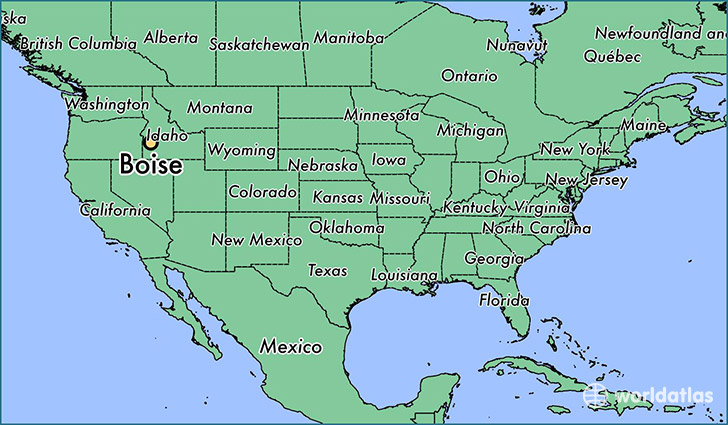
\includegraphics[width=0.8\textwidth]{images/boise-map.jpg}};

    \node [inner sep=0pt,,outer sep=0pt,clip,rounded corners=0.5cm] (ccp) at (3,-1){
      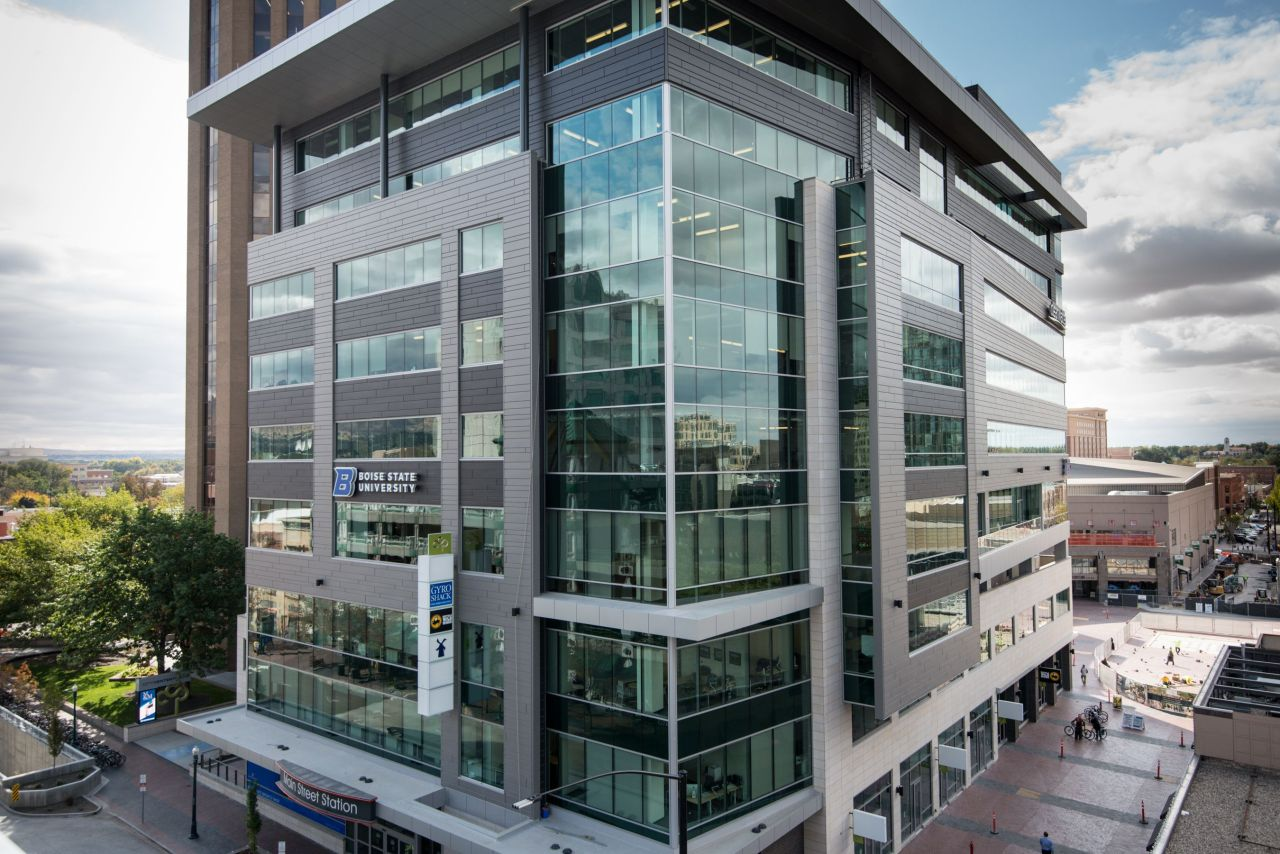
\includegraphics[width=0.45\textwidth]{images/CCP-from-northwest.jpg} };
    \draw[line width=4pt,
    arrows = {-Computer Modern Rightarrow[line cap=butt]}]       (ccp)   -- (-2.2,.8);

  \end{tikzpicture}

  \begin{block}{Boise State University}
    The Computer Science Department is located in Beautiful downtown Boise Idaho, United States!
  \end{block}

\end{frame}

\subsection{Our Research}


\begin{frame}
  \frametitle{Our Research}
  \begin{columns}
    \begin{column}{0.5\textwidth}
      We aim to find the current advances in using Rust in Kernel development to reduce the number of
      memory safety vulnerabilities in one of the most critical pieces of software that underpins all
      modern applications (SLR).
    \end{column}
    \begin{column}{0.5\textwidth}
      \begin{figure}
        \caption{A rusty computer\footnotemark[1]}
        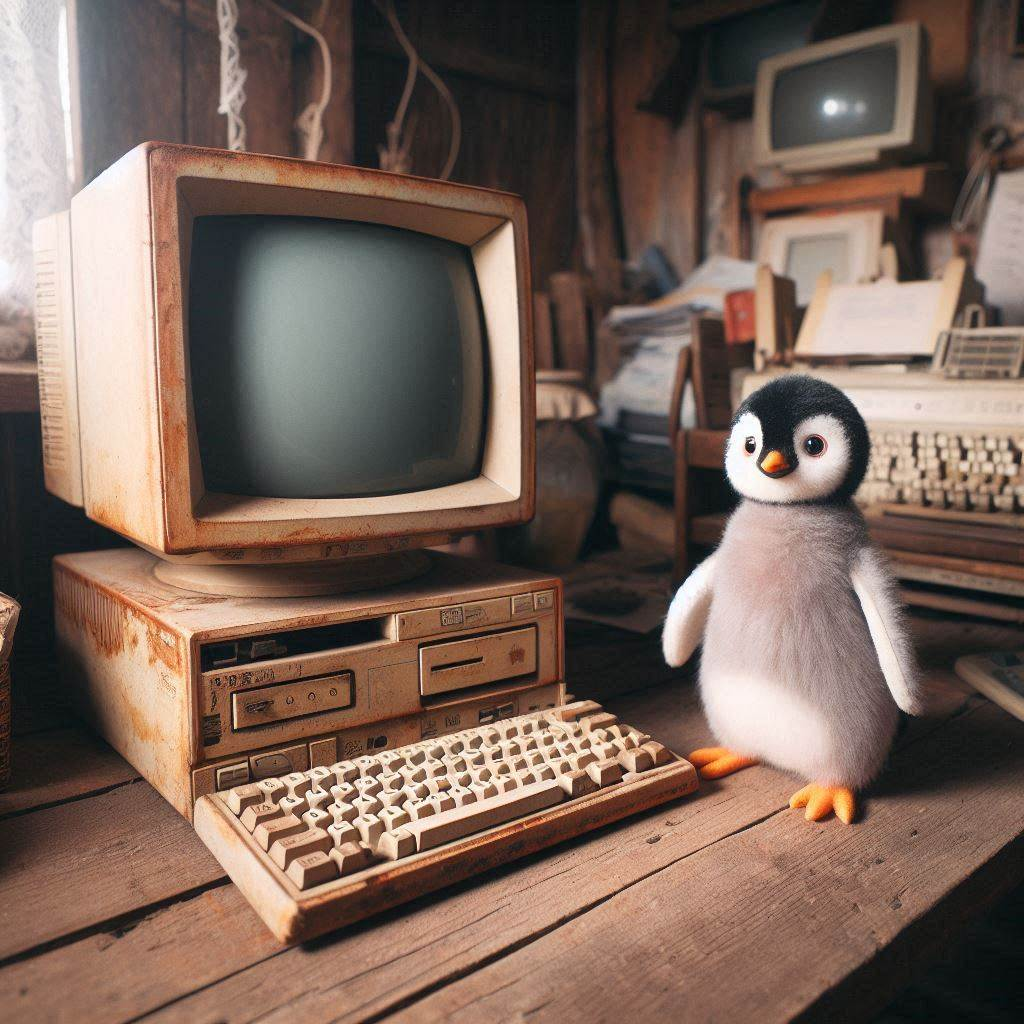
\includegraphics[width=.8\textwidth]{images/rusty.jpeg}\footnotemark[1]
      \end{figure}
    \end{column}
  \end{columns}
  \footnotetext[1]{AI Prompt: A rusty computer with a penguin next to it}
  \href{https://github.com/shanep/esem-2024/blob/master/proofs/esem24-50.pdf}{\beamergotobutton{Paper
    Link}}
\end{frame}

\section{Why Rust}
\begin{frame}
  \frametitle{Why Rust}
  \begin{itemize}
  \item<1-> Low-level \textbf{control} like C and C++
  \item<2-> Strong \textbf{safety} guarantees
  \item<3-> \textbf{Modern}, functional paradigms
  \item<4-> Industrial development and backing
  \item<5-> No garbage collector needed! All checks are performed at compile time
  \end{itemize}
\end{frame}

\section{Methodology}

\subsection{Research Questions}

\subsubsection{RQ1}
\begin{frame}
  \frametitle{RQ1}
  \begin{columns}
    \begin{column}{0.5\textwidth}
      \textbf{RQ1:} What are the existing approaches for implementing operating system kernels in Rust?\footnotemark[2]
    \end{column}
    \begin{column}{0.5\textwidth}
      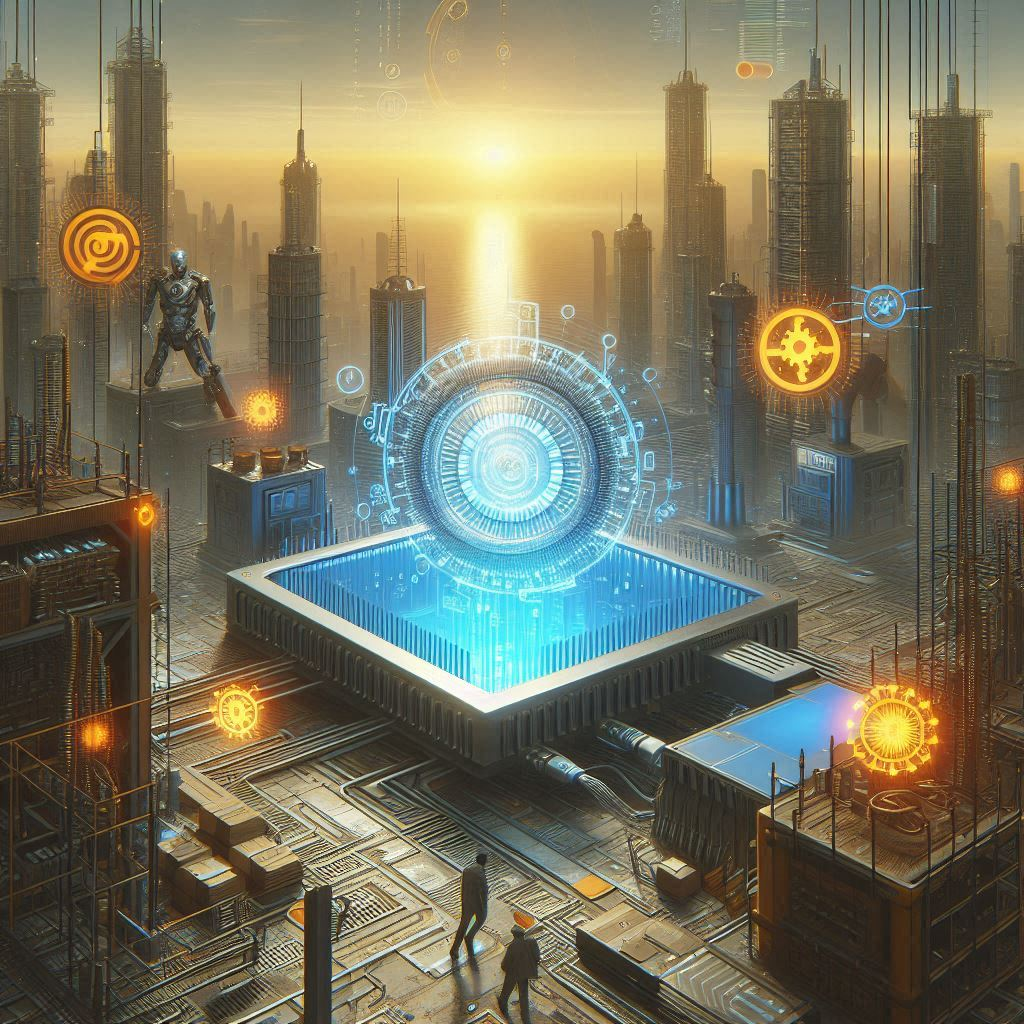
\includegraphics[width=.8\textwidth]{images/rq1.jpeg}
    \end{column}
  \end{columns}
  \footnotetext[2]{Fun side note: What happens if we put our research questions into an AI image generator?}
\end{frame}

\subsubsection{RQ2}
\begin{frame}
  \frametitle{RQ2}
    \begin{columns}
      \begin{column}{0.5\textwidth}
        \textbf{RQ2:} What are the performance implications of using Rust for operating system kernel development?
    \end{column}
    \begin{column}{0.5\textwidth}
      
\includegraphics[width=.8\textwidth]{images/rq2.jpeg}
    \end{column}
  \end{columns}
\end{frame}

\subsubsection{RQ3}
\begin{frame}
  \frametitle{RQ3}
  \begin{columns}
    \begin{column}{0.5\textwidth}
      \textbf{RQ3:} What are the major challenges and limitations when developing operating system kernels in Rust?
    \end{column}
    \begin{column}{0.5\textwidth}
      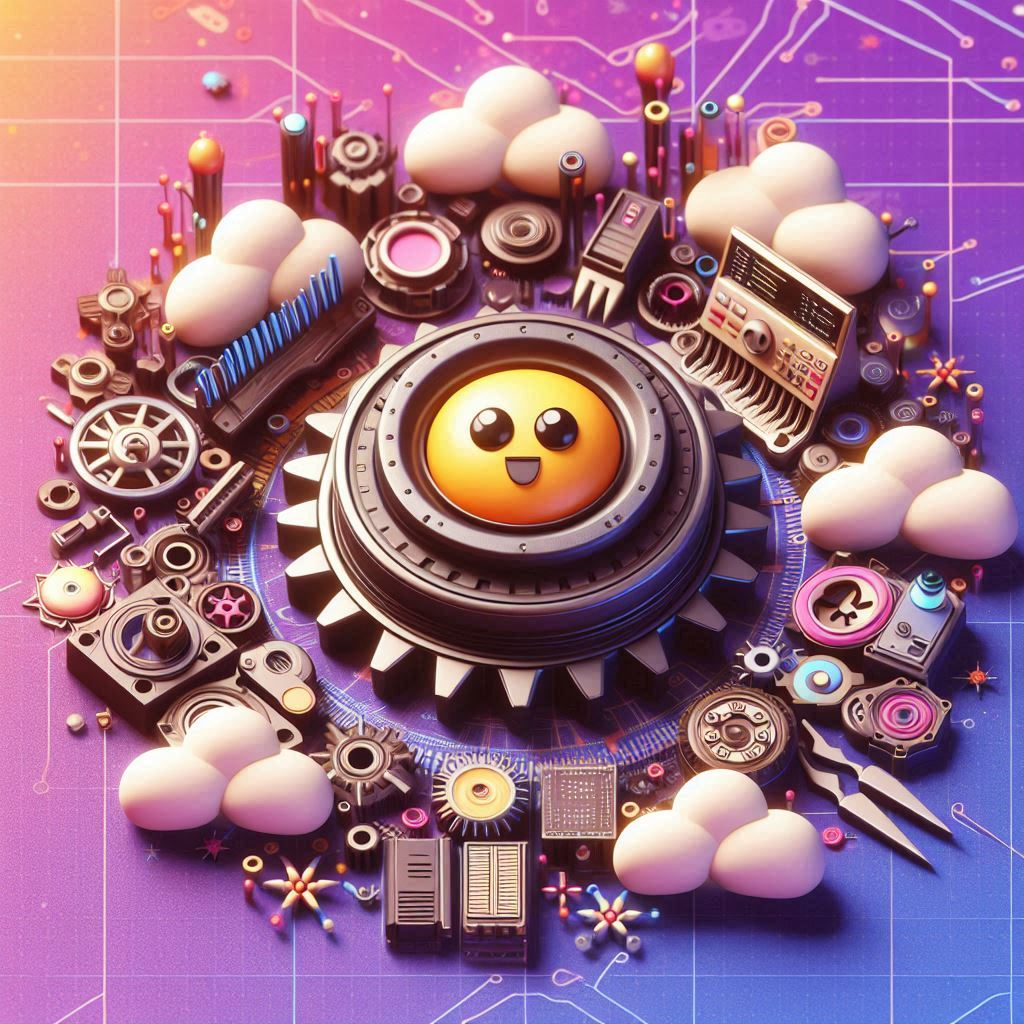
\includegraphics[width=.8\textwidth]{images/rq3.jpeg}
    \end{column}
  \end{columns}
\end{frame}

\subsubsection{RQ4}
\begin{frame}
  \frametitle{RQ4}
  \begin{columns}
    \begin{column}{0.5\textwidth}
      \textbf{RQ4:} What are the lessons learned when developing operating systems kernels in Rust?
      \end{column}
    \begin{column}{0.5\textwidth}
      
\includegraphics[width=.8\textwidth]{images/rq4.jpeg}
    \end{column}
  \end{columns}
\end{frame}

\subsection{Process Diagram}
\begin{frame}
  \frametitle{Process Diagram}
  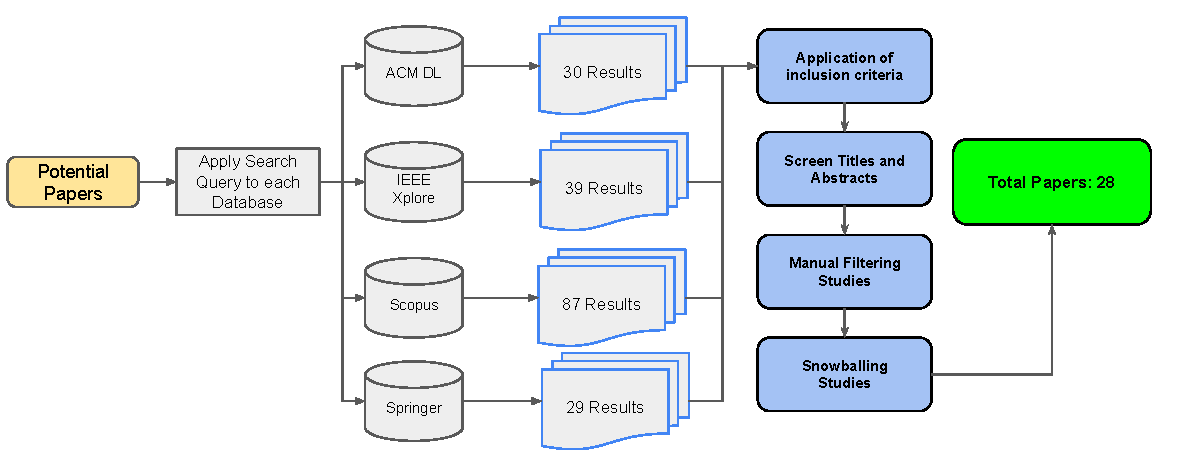
\includegraphics[width=4in]{figures/process-diagram.pdf}
\end{frame}
\section{Results}

\begin{frame}
  \frametitle{Results}
  \begin{columns}
    \begin{column}{0.5\textwidth}
      Our findings!
    \end{column}
    \begin{column}{0.5\textwidth}
      \begin{figure}
        \caption{Super happy researcher!\footnotemark[1]}
        
\includegraphics[width=.8\textwidth]{images/results.jpeg}\footnotemark[1]
      \end{figure}
    \end{column}
  \end{columns}
  \footnotetext[1]{AI Prompt: scientist getting research results and is super happy in a cyberpunk
    universe with lots of computers showing matrix code on them}
\end{frame}

\subsection{RQ1: Existing Approaches}
\begin{frame}
  \frametitle{RQ1}
  \begin{table}
    \caption{Approaches and Methodologies for Rust in the Kernel}
    \begin{tabular}{||l|l|l||}
      \hline
      Approach & Papers & Operating System in Rust\\
      \hline\hline
      Monolithic   & 4 & Linux Kernel v6.1+\\
      Micro-kernel & 5 & Atmosphere, Redox, Redleaf\\
      Embedded     & 2 & Tock, Hubris, Drone, Bern, HarSaRK \\
      Unikernel & 4 & RustyHermit, Theseus \\
       \hline
    \end{tabular}
    \label{tab:RQ1}
  \end{table}

\end{frame}

\subsection{RQ2: Performance Implications}
\begin{frame}
  \frametitle{RQ2}
  \begin{table}
    \caption{Performance Implications of Rust in the Kernel}
    \begin{tabular}{||l|l|l||}
      \hline
      No. & Implication & Studies that Reported the challenge\\
      \hline\hline
      1 & Performance & 3\\
      2 & Throughput & 1\\
      3 & Latency & 1 \\
      \hline
    \end{tabular}
    \label{tab:RQ2}
  \end{table}

  \begin{itemize}
  \item Performance issues - Caused by the safe $->$ unsafe transition layer
  \item Throughput issues - Caused by immature and or missing bindings within the FFI layer
  \item Latency issues - Caused by the interrupt layer written in Rust
  \end{itemize}

\end{frame}


\subsection{RQ3: Challenges and Limitations}
\begin{frame}
  \frametitle{RQ3: Challenges and Limitations}
  \begin{itemize}
  \item<1-> Binary Size
    \begin{itemize}
    \item Rust can produce larger binaries
    \item The same issue that C++ templates have!
    \end{itemize}
  \item<2-> Missing Features
    \begin{itemize}
    \item Rust still evolving and adding features
    \item Makes it difficult to integrate into the classroom due to the rapid evolution
    \end{itemize}
  \item<3-> Soundness - How to deal with raw memory without sacrificing safety?
  \item<4-> Panics - What happens when things go wrong?
  \item<5-> C Interop - Specific to mixed language kernels
  \end{itemize}
\end{frame}

\subsection{RQ4: Lessons Learned}

\begin{frame}
  \frametitle{RQ4: Lessons Learned}
  \begin{itemize}
  \item<1-> Impossible to use 100$\%$ rust - Same with C, some low level asm is needed to setup initial stack
    pointer, etc.
  \item<2-> Rust is not as expressive as other formal verification techniques
  \item<3-> Ownership root - An OS provides memory to rust so if the OS is itself written in rust
    who is the root owner?
    \begin{itemize}
    \item Open research question if this can even be done in software
    \item Researchers looking at hardware support (CHERI)
    \end{itemize}
  \end{itemize}

\end{frame}


\section{Conclusion}

\begin{frame}
  \frametitle{Conclusion}
  \begin{itemize}
  \item<1-> We are still in the early stages of figuring out who to do kernel dev in Rust
  \item<2-> High potential for enhanced security and stability
  \item<3-> Need to address integration issues (FFI)
  \item<4-> Need to expand the body of empirical evidence on Rust's impact! (Or more generally low
    level memory safe languages)
  \end{itemize}

\end{frame}

\section{Questions?}

\begin{frame}
  \frametitle{Questions?}
  \begin{columns}
    \begin{column}{0.5\textwidth}
      Questions?
    \end{column}
    \begin{column}{0.5\textwidth}
      \begin{figure}
        \caption{Happy People\footnotemark[1]}
        
\includegraphics[width=.8\textwidth]{images/questions.jpeg}\footnotemark[1]
      \end{figure}
    \end{column}
  \end{columns}
  \footnotetext[1]{AI Prompt: People attending a conference who all want to ask a question and are really excited!}
\end{frame}


\end{document}

%%% Local Variables:
%%% mode: LaTeX
%%% TeX-master: t
%%% End:
